\documentclass{article}

\usepackage[portuguese]{babel}

\usepackage{amsmath, amssymb}
\usepackage{graphicx}
\usepackage[colorlinks=true, allcolors=blue]{hyperref}

\usepackage[section]{placeins}

\title{Lista 01}
\author{Vinícius de Oliveira Peixoto Rodrigues (245294)}
\date{Agosto de 2022}

\begin{document}
\maketitle

\section*{Questão 1}

No script \texttt{playfair.py} em anexo se encontra uma implementação de decodificação do Playfair. A mensagem resultante é \texttt{"ODCAEHPARTEDAFEXEC"}, que é claramente \texttt{O DCA É PARTE DA FEEC} (o \texttt{X} apareceu porque há dois \texttt{E} repetidos).

\section*{Questão 2}

\subsection*{Item (a)}

\begin{itemize}
    \item Cada rotor tem 10 configurações iniciais (obtidas por meio de rotação), de modo que há $10^N = 10^4$ posições relativas entre os rotores (e, consequentemente, alfabetos distintos)
\end{itemize}

\subsection*{Item (b)}

\begin{itemize}
    \item Agora há $4!$ permutações entre os rotores, de modo que há agora $4! \cdot 10^4$ alfabetos
\end{itemize}

\subsection*{Item (c)}

\begin{itemize}
    \item Como não pode haver rotores iguais, o número máximo é de 10 rotores, de modo que resultam $10! \cdot 10^{10}$ alfabetos
\end{itemize}

\section*{Questão 3}

O efeito avalanche é a propriedade de uma ferramenta criptográfica de produzir mudanças drásticas no saída mediante pequenas mudanças na entrada. 

Existe também um critério de avalanche mais formal e probabilístico, que é satisfeito quando a mudança de um bit na entrada faz com que cada bits da saída tenha 50\% de chance de trocar.

Esse efeito é definido (e desejável) tanto em relação à chave quanto ao texto de entrada, visto que se tanto um quanto o outro não exibissem esse efeito, seria possível se aproveitar da correlação entrada-saída como via de ataque estatístico.

\section*{Questão 4}

    Suponha que um atacante consiga acesso ao \textit{comprimento} da chave. Usaremos como exemplo a chave \texttt{carta}, de comprimento 5, que será usada para cifrar um fragmento ($\approx$ 4.5k palavras) do primeiro capítulo de \textit{"A Hora da Estrela"}, de Clarice Lispector. Todos os resultados apresentados aqui foram gerados a partir do script \texttt{vigenere.py}, que se encontra em anexo.

    Conhecendo-se o $k$ da chave, sabe-se imediatamente que todos os caracteres a uma distância múltipla de $k$ uns dos outros foram cifrados com a mesma cifra de César (visto que cada linha da tabela de Vigenere é uma cifra de César com offset igual à distância de um caractere da cifra até o \texttt{'a'}). Desse modo, é possível estudar a distribuição de frequências para esses grupos. A imagem abaixo mostra a distribuição para o grupo com os caracteres na posição 1, 6, 11, 16, ...

    \newpage
    \FloatBarrier
    \begin{figure}[!ht]
        \begin{center}
            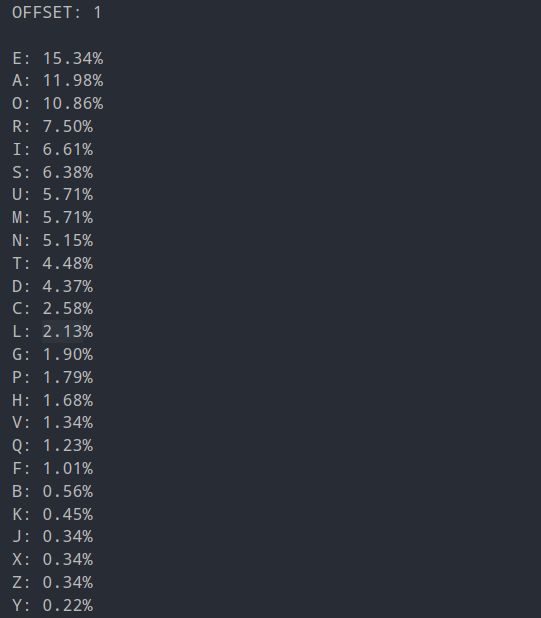
\includegraphics[width=\textwidth]{images/q4_1.png}
            \caption{Distribuição de frequência dos caracteres em posições $\equiv 1 \mod{5}$}
        \end{center}
    \end{figure} 

    Da tabela, é possível perceber que há um grupo de três caracteres mais frequentes que os demais. Os dados para todos os grupos apresentam essa regularidade (e estão em anexo no arquivo \texttt{vigenere\_statistics.txt}).

    Na \href{https://pt.wikipedia.org/wiki/Frequ%C3%AAncia_de_letras}{Wikipedia}, é possível encontrar uma tabela de frequência de letras no português:

    \newpage
    \FloatBarrier
    \begin{figure}[!ht]
        \begin{center}
            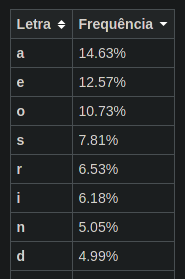
\includegraphics[width=0.4\textwidth]{images/q4_2.png}
            \caption{Frequência de letras no português}
        \end{center}
    \end{figure} 

    A partir desses dados, que nos informa que o grupo das três letras com frequência mais alta são \texttt{a, e, o}, é possível descobrir a chave.
    
    Por exemplo, seguindo os dados da Figura 1, vemos imediatamente que o grupo \texttt{e, a, o} tem a frequência mais alta, de modo que o caractere na posição 1 da chave deve ser \texttt{\_a\_\_\_}.

    \FloatBarrier
    \begin{figure}[!ht]
        \begin{center}
            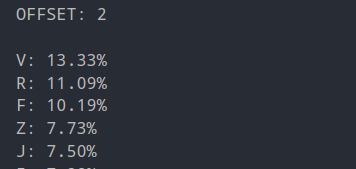
\includegraphics[width=0.4\textwidth]{images/q4_3.png}
            \caption{Frequência de letras em posições $\equiv 2 \mod{5}$}
        \end{center}
    \end{figure} 

    Do grupo acima, vemos que \texttt{v, r, f} deve corresponder a alguma permutação de \texttt{a, o, e}. Analisando com cuidado:

    \begin{itemize}
        \item \texttt{'o' - 'a' = 14}
        \item \texttt{'o' - 'e' = 10}
        \item \texttt{'e' - 'a' = 4}
    \end{itemize}

    Comparando com grupo cifrado:

    \begin{itemize}
        \item \texttt{'v' - 'r' = 4} $\Rightarrow$ \texttt{'a' -> 'r'}, \texttt{'e' -> 'v'}
    \end{itemize}

    De modo que se encontra mais um caractere da chave: \texttt{\_ar\_\_\_}

    Por meio desse processo é possível quebrar a chave inteira.

    \section*{Questão 5}

    O one-time pad é uma extensão natural da cifra de Vigenere, visto que a vulnerabilidade descrita na questão anterior advém do fato de a chave ter tamanho menor que o texto e portanto ter que ser concatenada, fazendo com que porções igualmente espaçadas do texto sejam cifradas "juntas". Essa regularidade é eliminada no one-time pad, onde se use uma chave aleatória do tamanho do texto (de modo que a ausência de um padrão estatístico na chave implica na ausência de um padrão estatístico no texto cifrado).

    \section*{Questão 6}

    Os alemães, durante a Segunda Guerra, usavam 5 aspectos do \textit{Enigma} como chaves:
    \begin{itemize}
        \item A ordem dos rotores
        \item A posição do anel ajustável do alfabeto em relação à fiação cada rotor
        \item As conexões no \textit{plugboard} da máquina
        \item A configuração do refletor reconfigurável
        \item A posição inicial dos rotores
    \end{itemize}

    Todos esses fatores juntos funcionam como a "chave" da cifra.
    
    \section*{Questão 7}

    Difusão e confusão são dois conceito relacionados que têm origem nos trabalhos de Claude Shannon, pai da Teoria da Informação.

    \begin{itemize}
        \item \textbf{Difusão} se refere ao obscurecimento de traços estatísticos do texto em claro no texto cifrado. Isso normalmente é alcançado por meio de várias iterações seguidas de operações de  "embaralhamento", como substituição e permutação (por exemplo, na permutação das S-boxes do DES e no ShiftRows/MixColumns do AES). Serve para prevenir ataques estatísticos.
        \item \textbf{Confusão} se refere a tornar a relação entre a chave e o texto cifrado o mais complexa e imprevisível possível. Isso é importante para garantir que mesmo com um número muito grande de pares P-C, ainda seja muito difícil obter informação sobre a chave.
    \end{itemize}

    \section*{Questão 8}

    Ataques estatísticos tomam vantagem de deficiências de difusão para encontrar informação sobre chaves (ou até sobre o próprio texto em claro) a partir da análise estatística do texto cifrado. Um exemplo é a sequência de passos apresentada na Questão 4 para quebrar a cifra de Vigenere.

    Como mencionado na Questão 7, o uso de algoritmos criptográficos com alta difusão torna difícil o ataque estatístico.

    \section*{Questão 9}

    Dados:

    Meu nome: \texttt{VINICIUSDEOLIVEIRAPEIXOTORODRIGUES} (comprimento 34)

    Meu RA: \texttt{245294} $\rightarrow$ \texttt{k1 = 4}

    \texttt{k2 = 7 2 1 8 3 0 5 6 4}

    \subsection*{Cifrar}
    
    Inicialmente:
    \begin{center}
    \begin{tabular}{|c|c|c|c|c|c|c|c|c|}
       \hline
       \textbf{0} & \textbf{1} & \textbf{2} & \textbf{3} & \textbf{4} & \textbf{5} & \textbf{6} & \textbf{7} & \textbf{8} \\
       \hline
       v & i & n & i & c & i & u & s & d \\ \hline
       e & o & l & i & v & e & i & r & a \\ \hline
       p & e & i & x & o & t & o & r & o \\ \hline
       d & r & i & g & u & e & s & 0 & 0 \\ \hline
    \end{tabular}
    \end{center}

    Em seguida, concatenamos as colunas na ordem da chave:

    Resultado: \texttt{"SRR0NLIIIOERDAO0IIXGVEPDIETEUIOSCVOU"}

    \begin{center}
    \begin{tabular}{|c|c|c|c|c|c|c|c|c|}
       \hline
       s & n & i & d & i & v & i & u & c \\ \hline
       r & l & o & a & i & e & e & i & v \\ \hline
       r & i & e & o & x & p & t & o & o \\ \hline
       0 & i & r & 0 & g & d & e & s & u \\ \hline
    \end{tabular}
    \end{center}


    \subsection*{Decifrar}

    Para decifrar, calculamos o número de colunas dividindo o tamanho da cifra pela chave \texttt{k1}: \texttt{36/4 = 9}, de modo que temos os grupos

    \begin{center}
    \begin{tabular}{|c|c|c|c|c|c|c|c|c|}
       \hline
       \textbf{7} & \textbf{2} & \textbf{1} & \textbf{8} & \textbf{3} & \textbf{0} & \textbf{5} & \textbf{6} & \textbf{4} \\
       SRR0 & NLII & IOER & DAO0 & IIXG & VEPD & IETE & UIOS & CVOU \\ \hline
    \end{tabular}
    \end{center}

    Reorganizando novamente em colunas de acordo com as posições na chave:

    \begin{center}
    \begin{tabular}{|c|c|c|c|c|c|c|c|c|}
       \hline
       v & i & n & i & c & i & u & s & d \\ \hline
       e & o & l & i & v & e & i & r & a \\ \hline
       p & e & i & x & o & t & o & r & o \\ \hline
       d & r & i & g & u & e & s & 0 & 0 \\ \hline
    \end{tabular}
    \end{center}

    De onde obtemos de volta o texto em claro
    
    \texttt{"VINICIUSDEOLIVEIRAPEIXOTORODRIGUES"}.

    \section*{Questão 10}

    Partindo-se do pressuposto que o algoritmo criptográfico usado é conhecido pelo atacante (princípio conhecido como máxima de Shannon), é possível delinear algumas categorias:

    \begin{itemize}
        \item Texto cifrado conhecido, quando o atacante só tem acesso a um conjunto (potencialmente grande) de texto encriptado
        \item Texto em claro conhecido, quando o atacante tem acesso a um conjunto de pares P-C
        \item \textit{Chosen-plaintext/chosen-ciphertext}, quando o atacante consegue obter texto cifrado a partir de texto em claro conhecido ou vice-versa
        \item \textit{Adaptive chosen-plaintext/chosen-ciphertext}, quando o atacante escolhe premeditadamente textos em claro baseado em informações obtidas de ciframentos anteriores
    \end{itemize}

\end{document}
